\startappendix{Appendix}
\label{ch:appendix}


\begin{figure}[!ht]
\centering
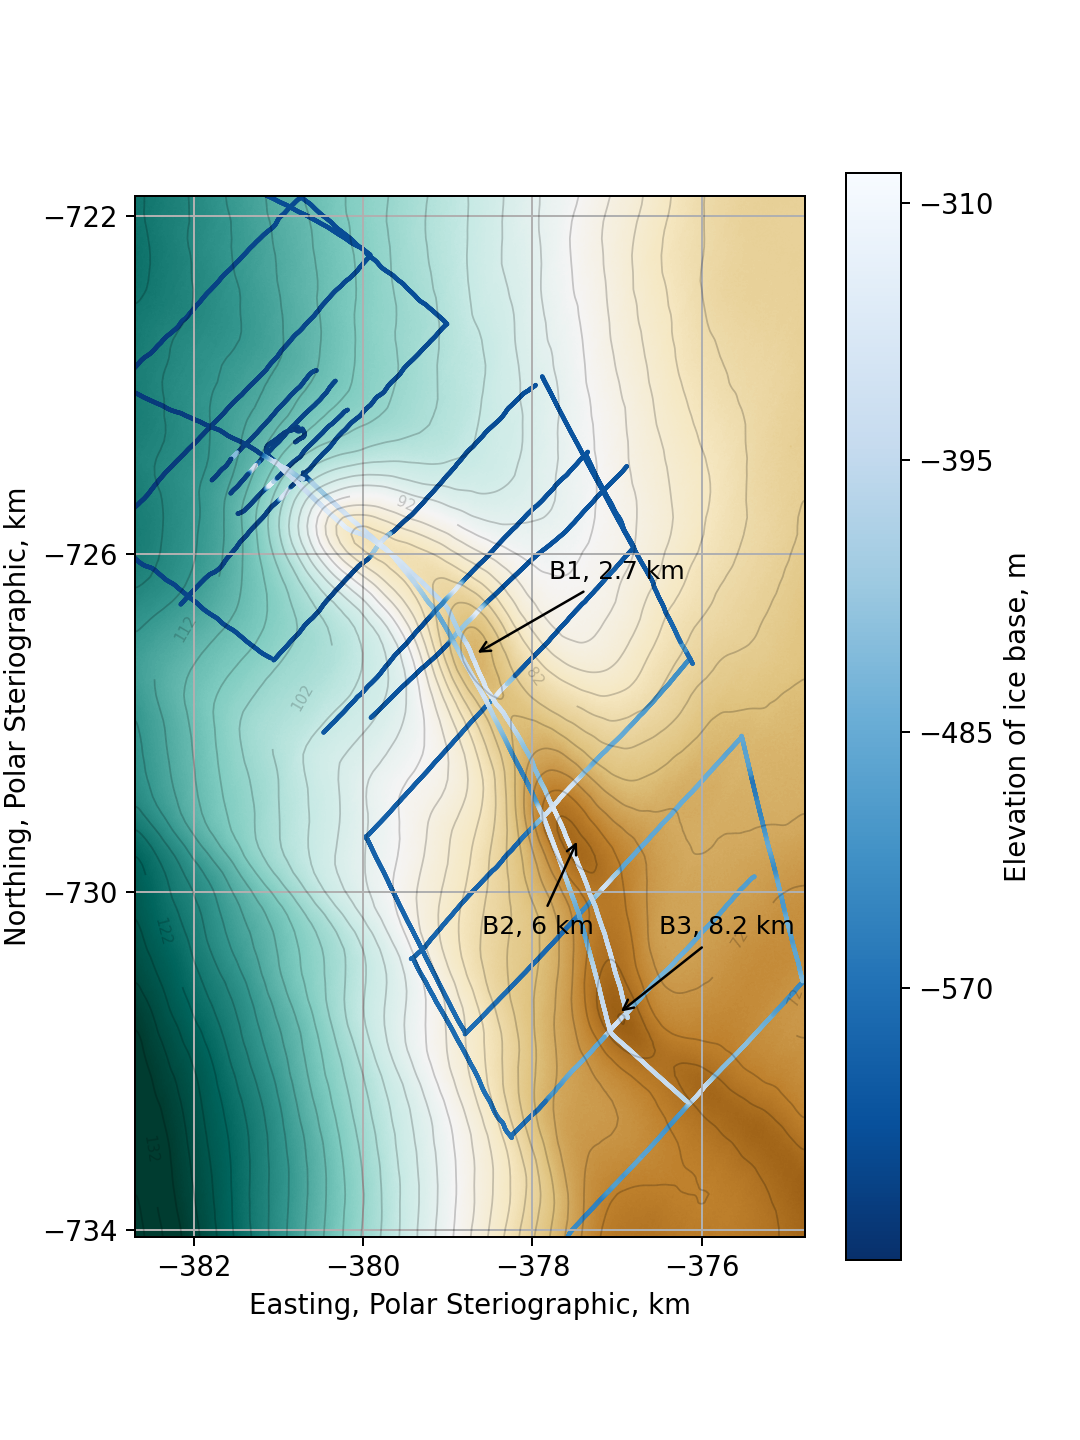
\includegraphics[width=0.8\textwidth]{chapters/2/radarlines_surfcolour.png}
\caption[Radar line depths]{Ice depths picked from processed radar data. Note that the channel forms over a short distance.}
\label{fig:radarlines_surfcoloure}
\end{figure}



\begin{figure}[h!]
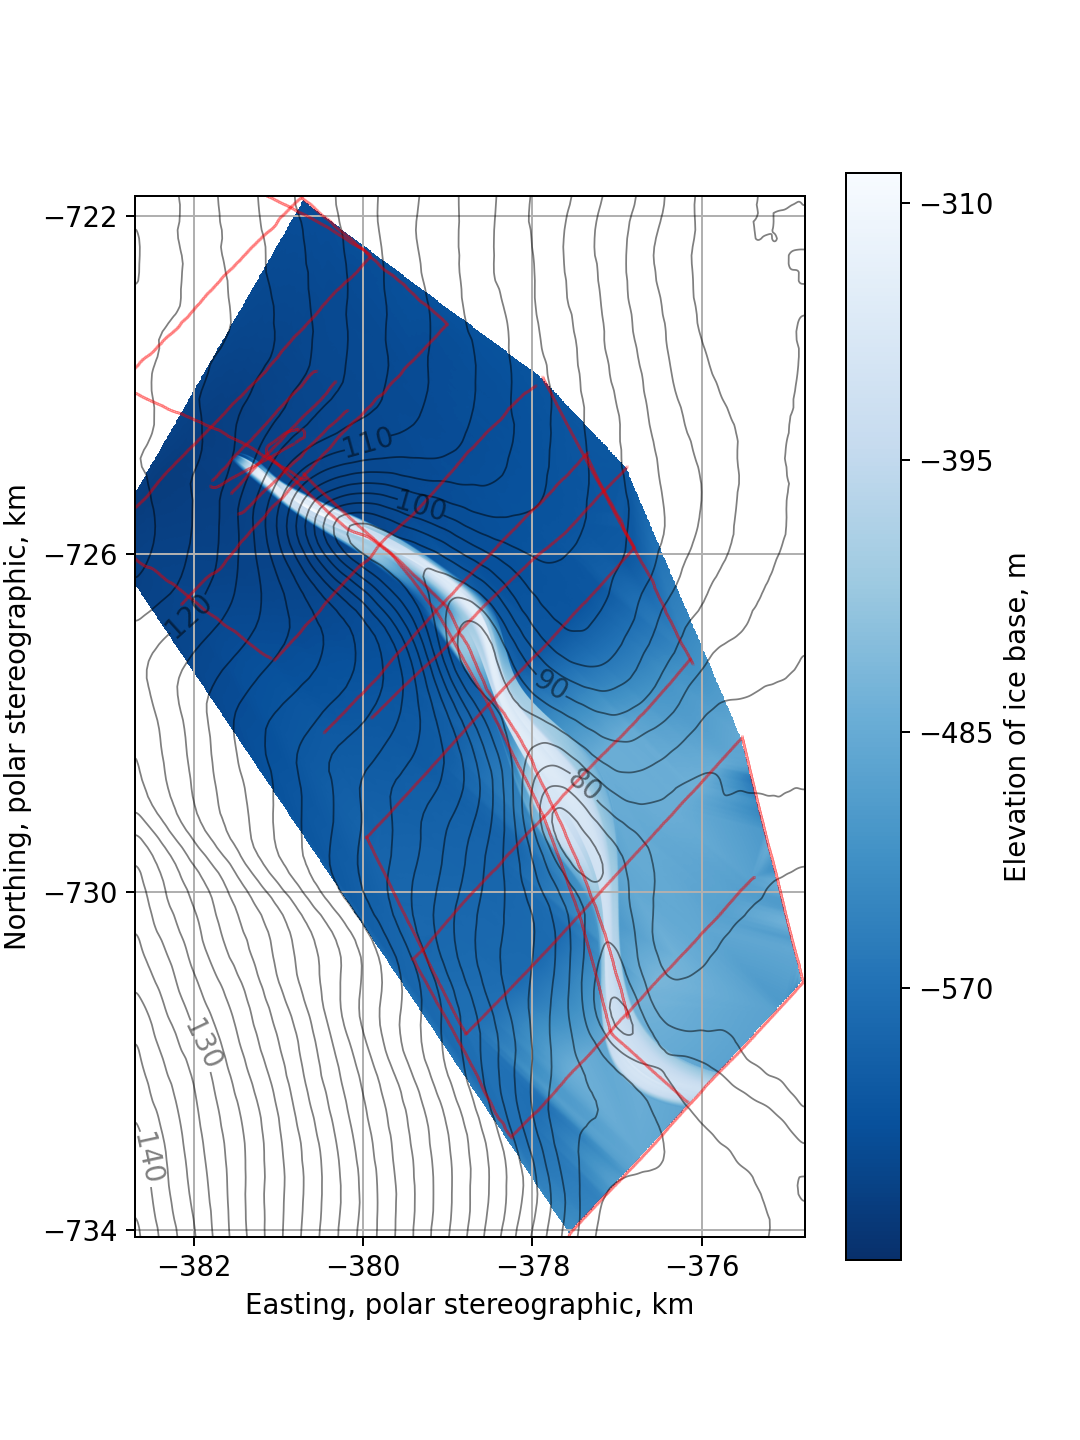
\includegraphics[width=1\textwidth]{chapters/2/ice_base_solo.png}
 \caption[Ice base map]{Image shows ice base elevation estimated using downstream interpolation described in Section 2.2.2. Red lines show location of radar data collection which informed the interpolation. Contours are REMA ice surface elevation \cite{howat2019reference}.
% The three lines extending out the bottom of the plot are radar data from operation ice bridge \cite{studinger2010operation}, and other other lines are from the 15-16 preliminary radar survey. 
}
\label{fig:ice_base_solo}
\end{figure}
%
\begin{figure}[ht!]
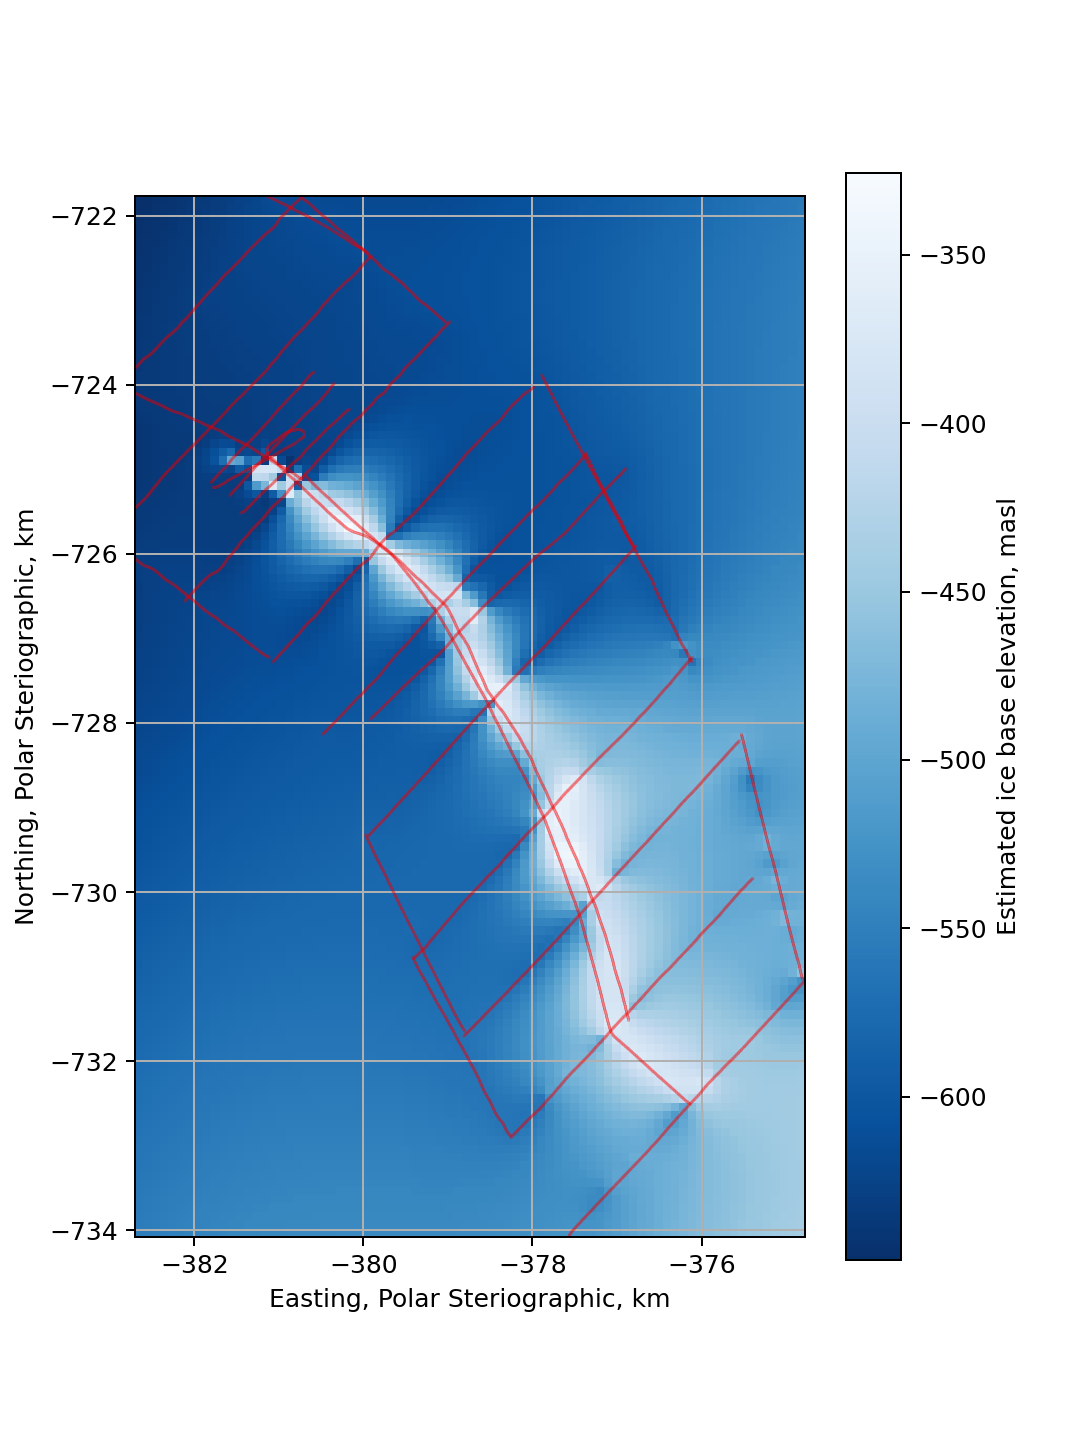
\includegraphics[width=1\textwidth]{chapters/2/gmt_surface_interp.png}
\caption[Ice base poor interpolation]{Ice base elevation estimated using continuous curvature spline interpolation. Red lines show radar data which was interpolated. The interpolation does not produce a good result, showing clear bias to surveyed locations.}
\label{fig:gmt_surface_interp}
\end{figure}

\begin{figure}[!ht]
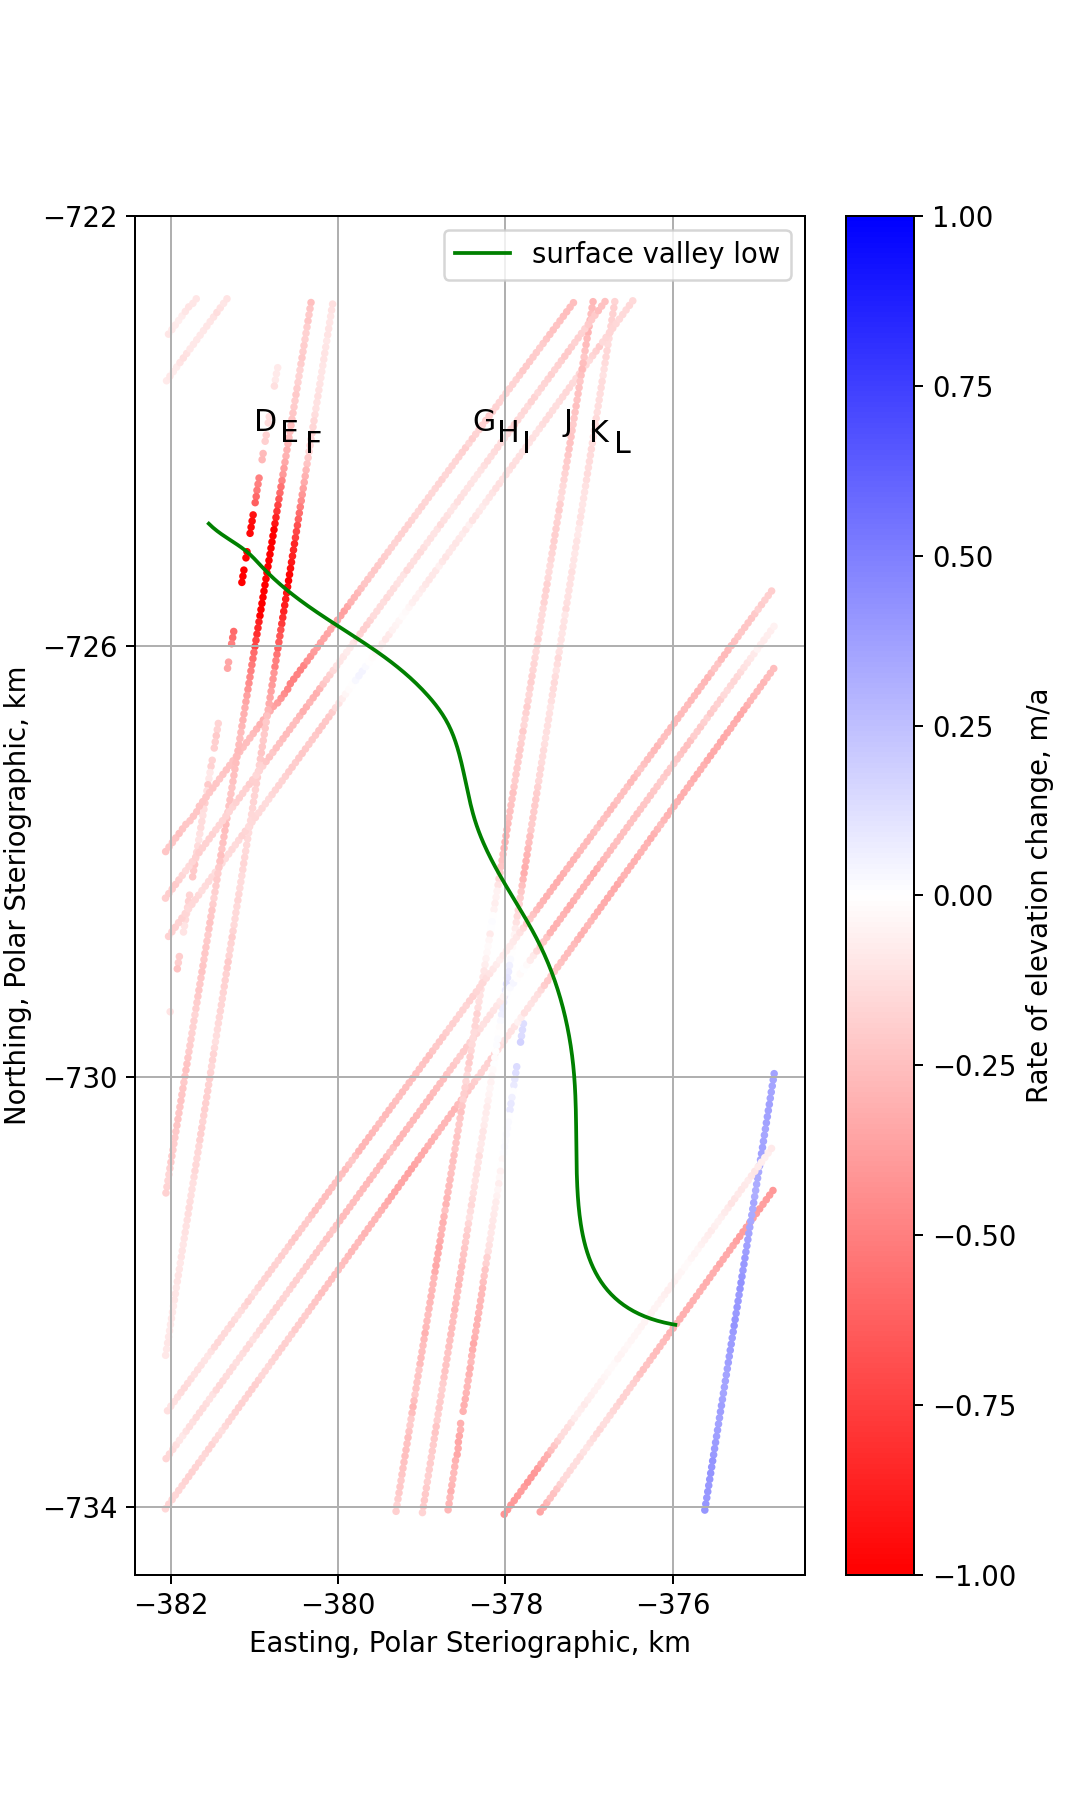
\includegraphics[width=0.9\textwidth]{chapters/2/icesat2_a.png}
\caption[ICESat--2 plan view]{Map showing surface elevation changes with ICESat--2 data. Letters D-L refer to the locations of cross sections shown in Figure 10.}
\label{fig:icesat2_a}
\end{figure}
  %
\begin{figure}[!ht]
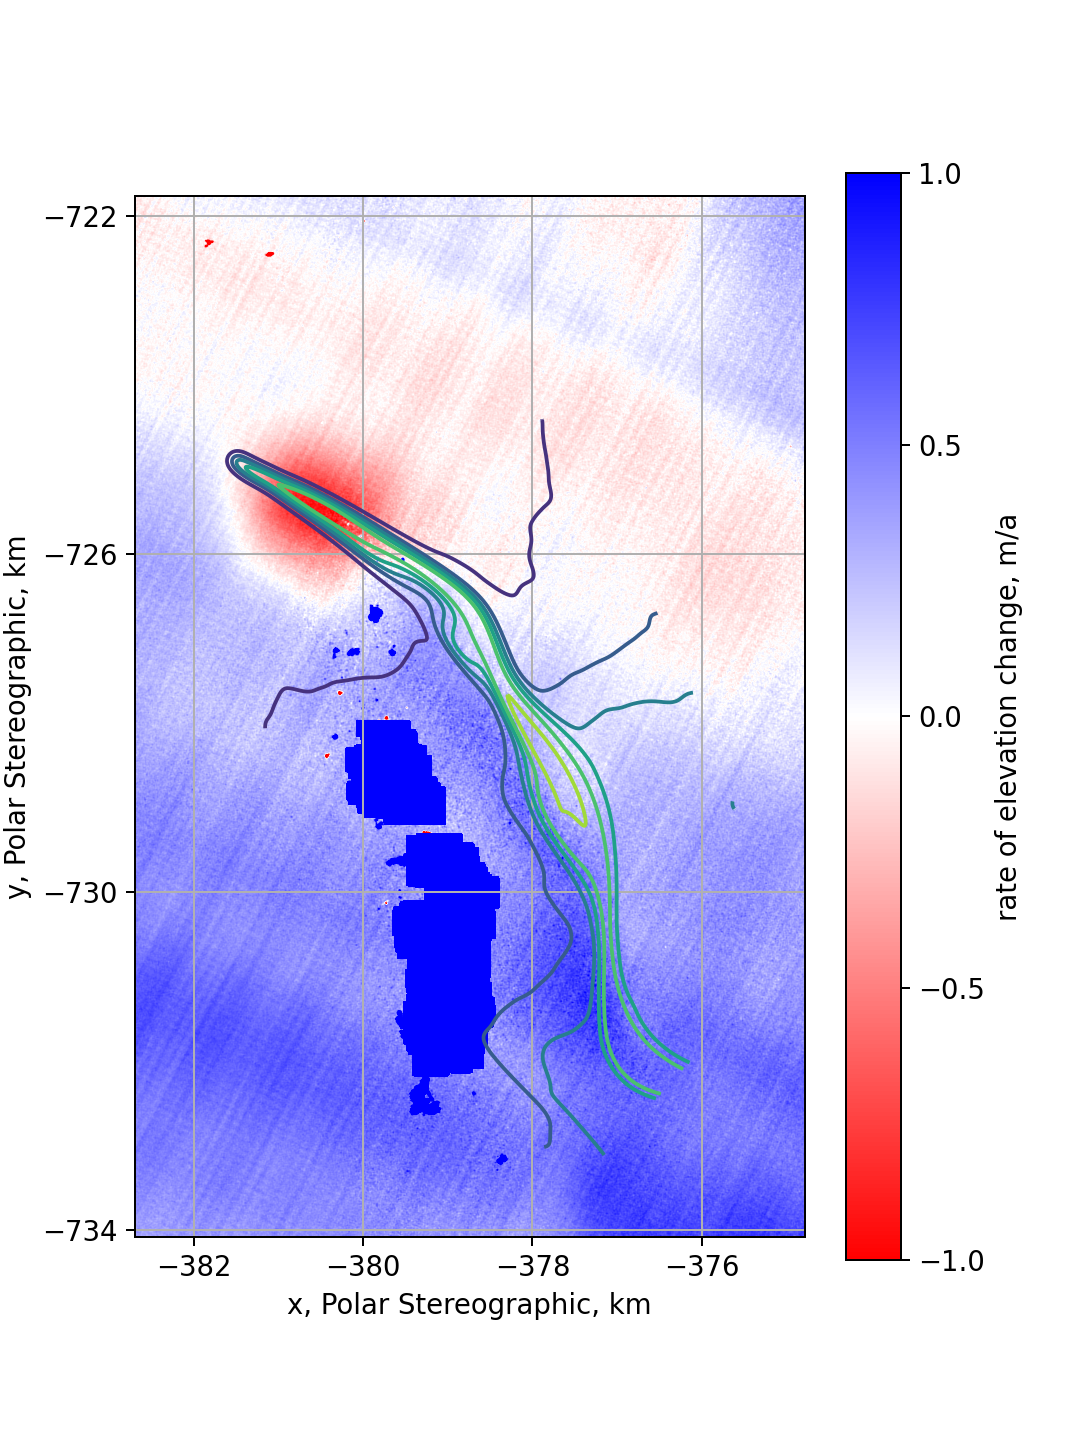
\includegraphics[width=1\textwidth]{chapters/2/REMAdiff_alone.png}
\caption[REMA difference map]{Difference between REMA elevation from 2012-12-24 to 2016-11-09, contours show estimated ice base. Dark blue spots to the true--right of the channel are artefacts.}
\label{fig:REMAdiff_alone.png}
\end{figure}



\begin{figure}[!ht]
\centering
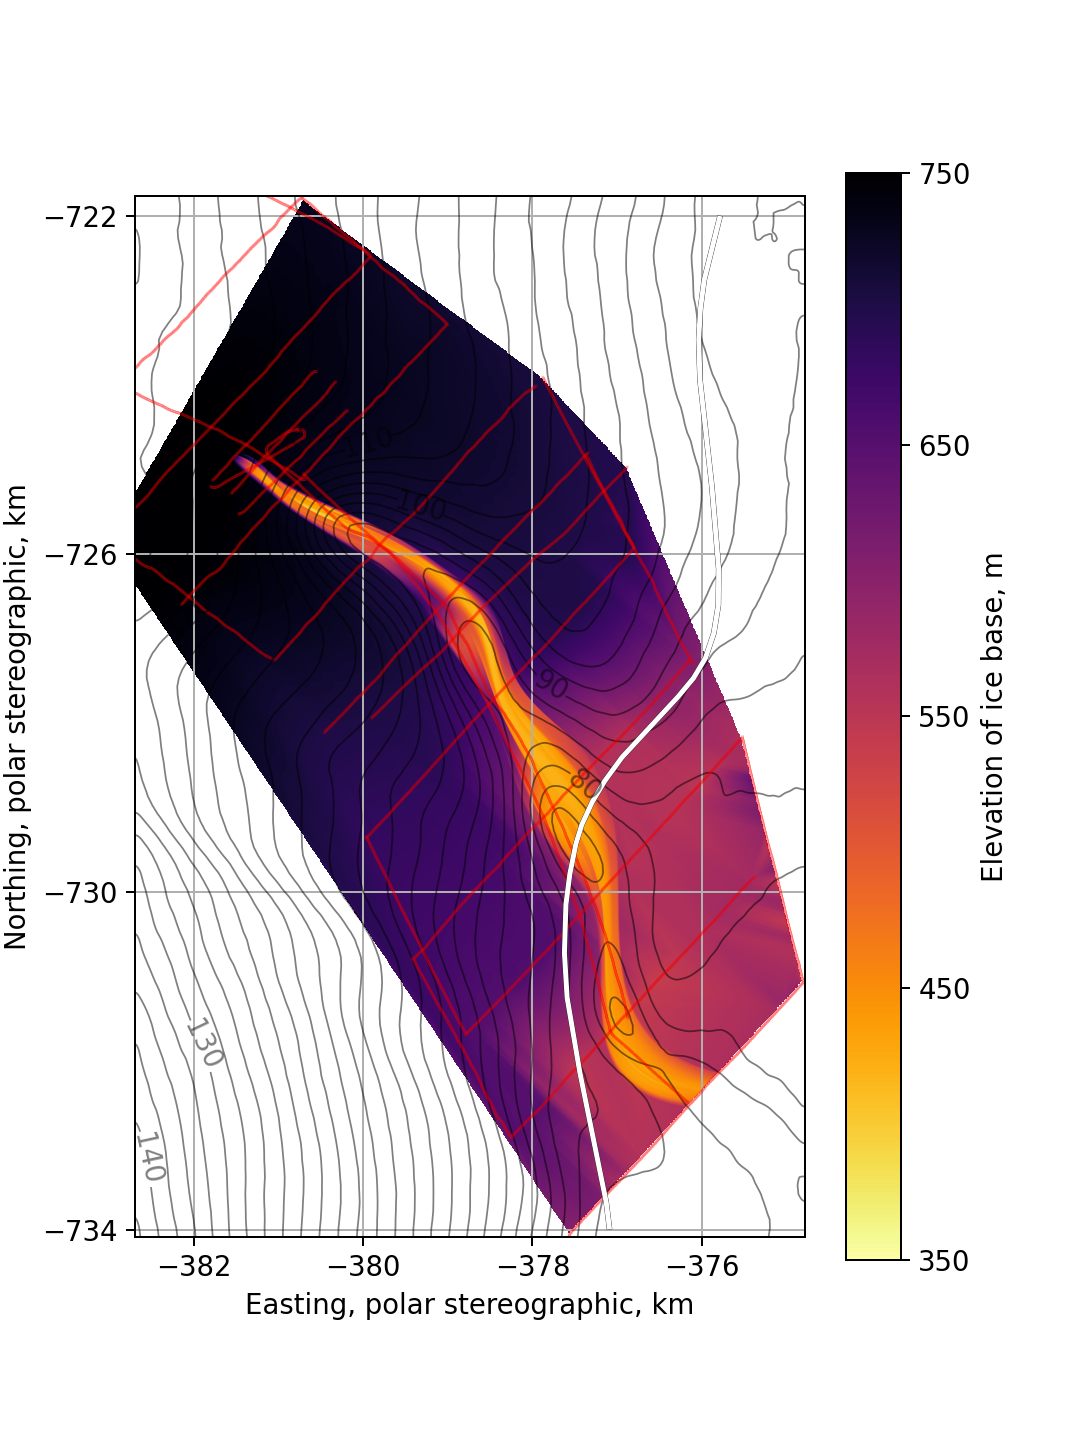
\includegraphics[width=1.1\textwidth]{chapters/2/thickness_solo.png}
\caption[Ice thickness]{Image shows ice thickness estimated using downstream interpolation described in Section 2.2.2. Red lines show location of radar data collection which informed the interpolation. Contours are REMA ice surface elevation \cite{howat2019reference}.}
\label{fig:thickness_solo}
\end{figure}



\begin{figure}[!ht]
\centering
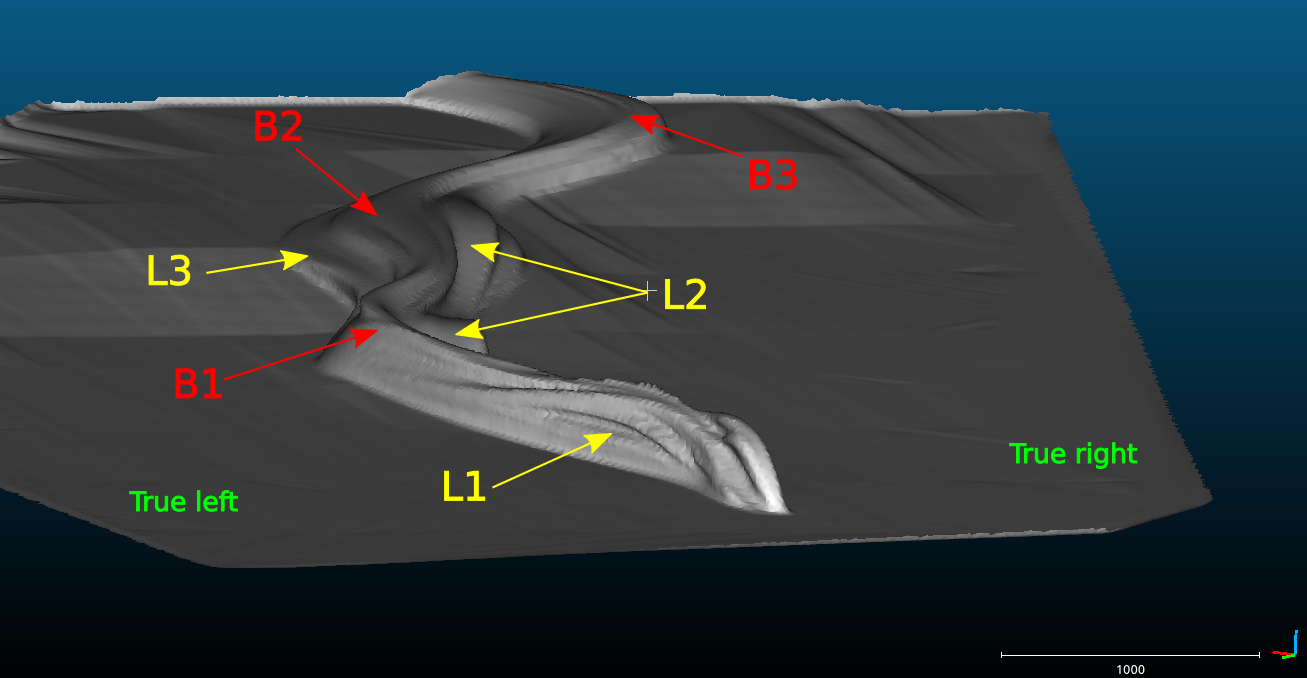
\includegraphics[width=1.1\textwidth]{chapters/2/ledges1.png}
\caption[3D ledge view (A)]{Three dimensional view of the ice base map, showing the location of ledges (L1, L2, L3) and bends in the channel (B1, B2, B3). Bends correspond to basins on the subaerial ice surface.}
\label{fig:ledges1}
\end{figure}

\begin{figure}[!ht]
\centering
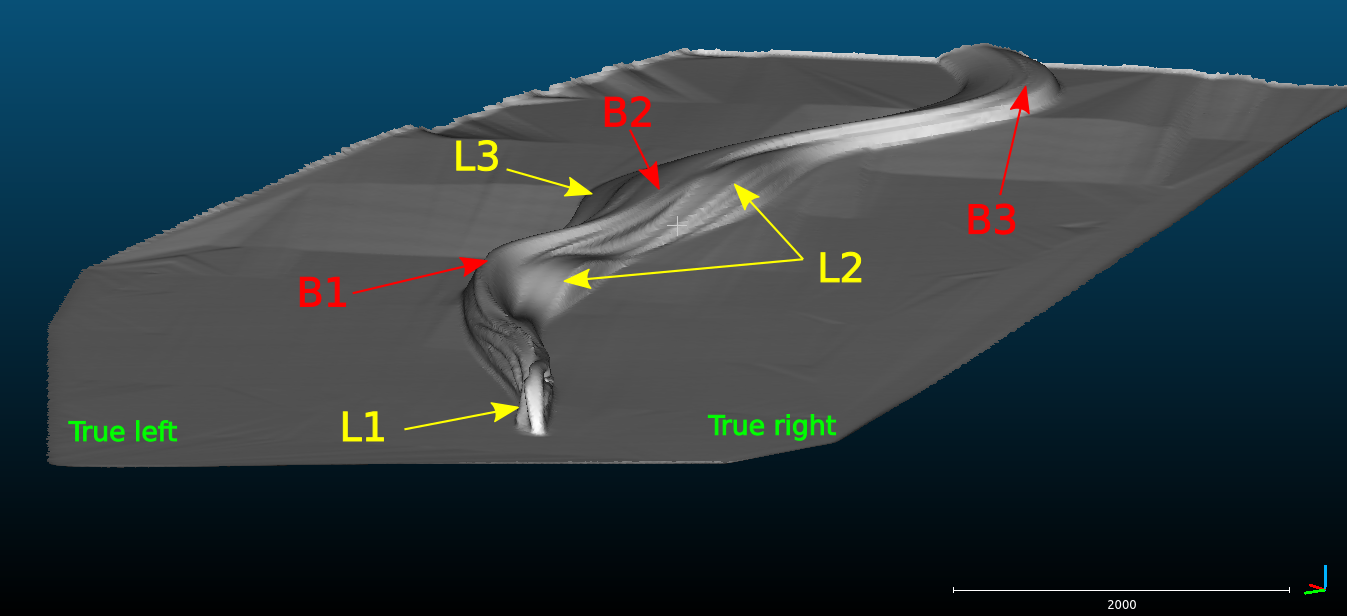
\includegraphics[width=1.1\textwidth]{chapters/2/ledges2.png}
\caption[3D ledge view (B)]{Three dimensional view of the ice base map, showing the location of ledges (L1, L2, L3) and bends in the channel (B1, B2, B3). Bends correspond to basins on the subaerial ice surface.}
\label{fig:ledges2}
\end{figure}

\begin{figure}[!ht]
\centering
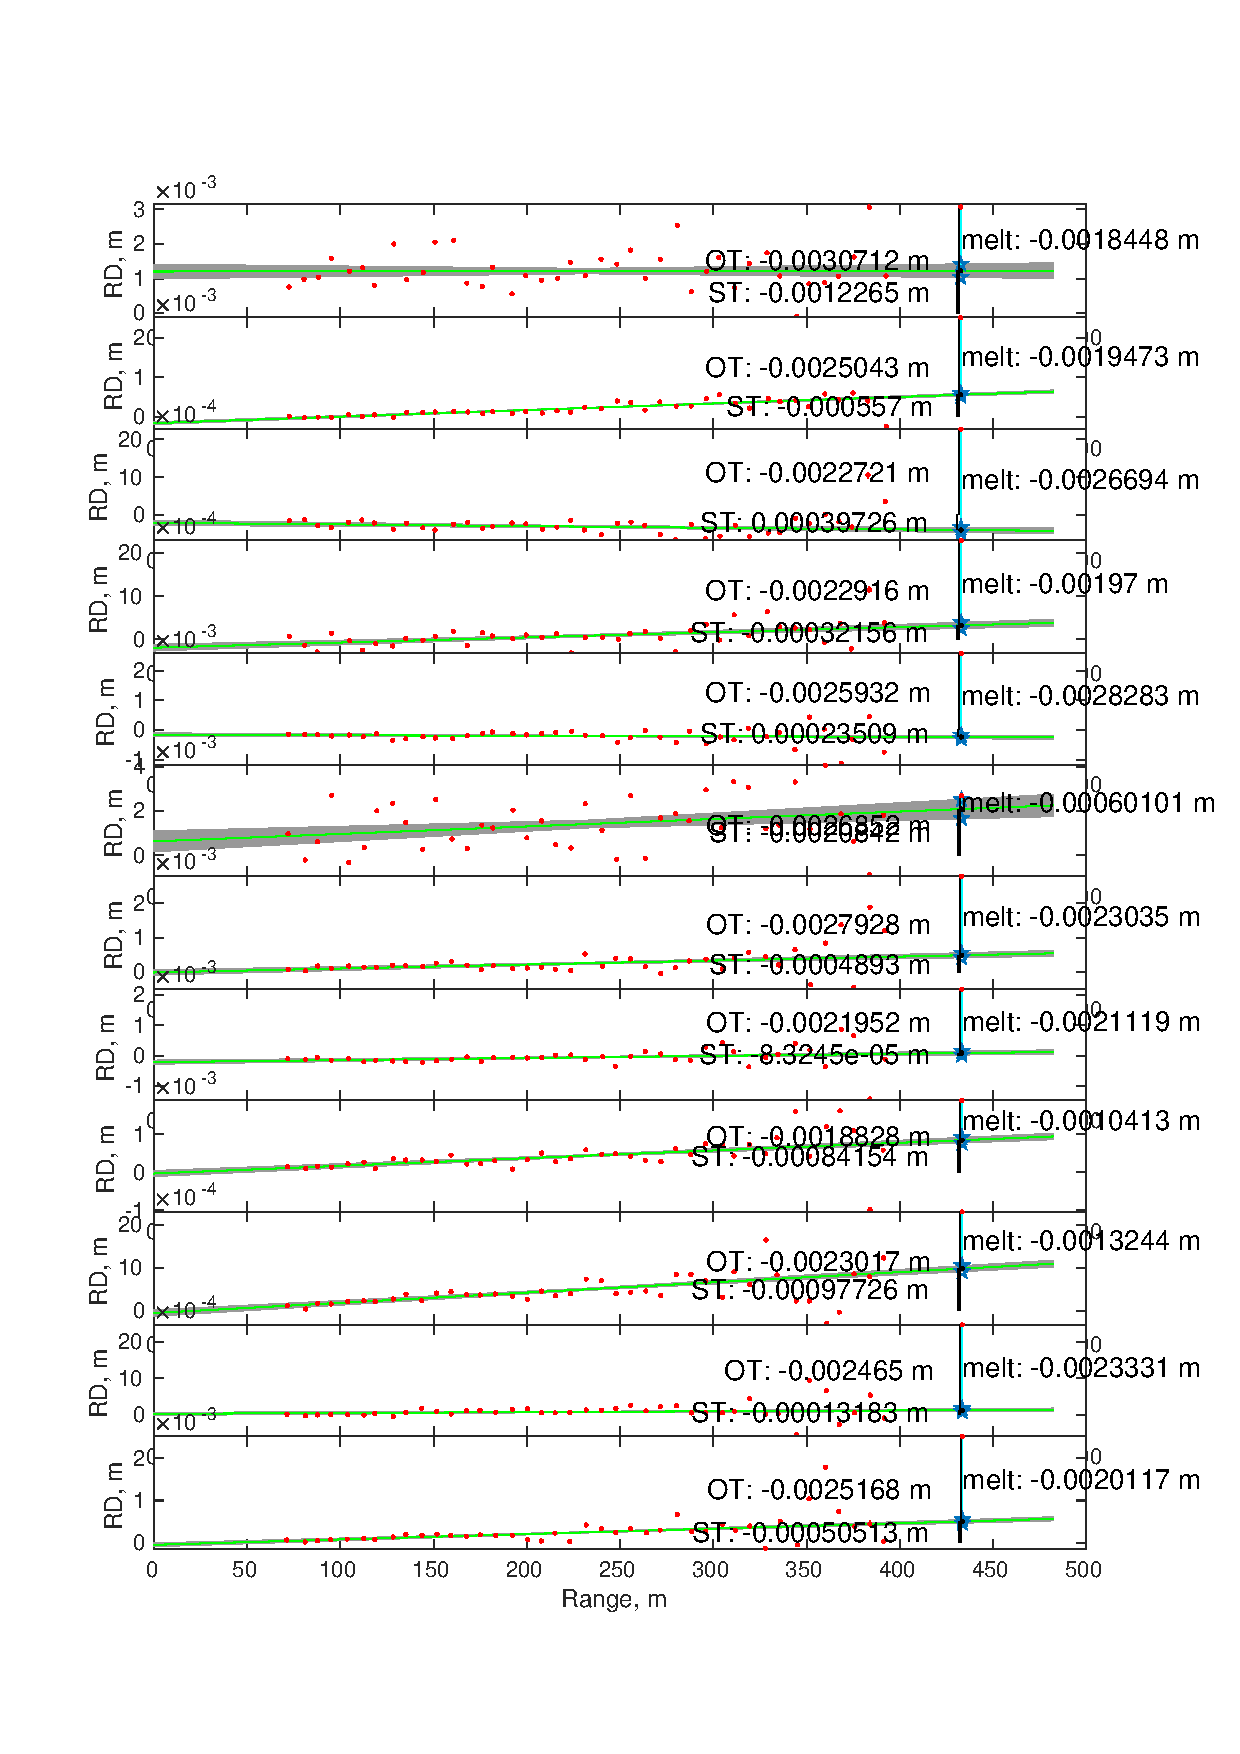
\includegraphics[width=0.7\textwidth]{chapters/3/12strains.pdf}
\caption[Monthly strain]{As in Figure \ref{fig:range_amp_phase}, 12 separate ApRES observations are shown over 12 months of 2020. Range difference of internal reflectors (red points) over a 28 hour interval centred on the 1st of each month of 2020.  Top plot is from January, bottom plot from December.  RD (y-axis) is range difference, OT is observed thinning, ST is strain thinning. Green area shows one standard deviation of a linear fit of the internal reflectors. Melt is the negative of apparent accretion.
% C) Line of best fit through change in internal reflectors.
}
\label{fig:12strains}
\end{figure}

\begin{figure}[!ht]
\centering
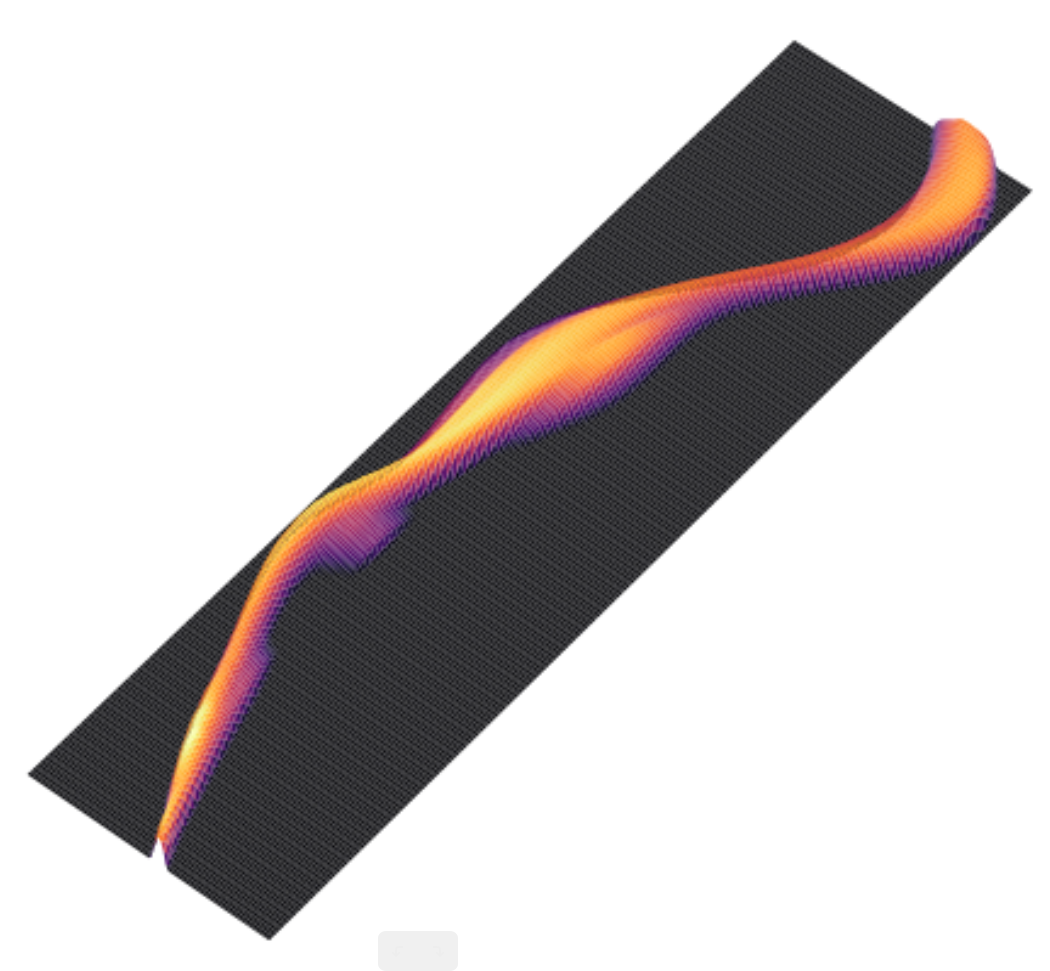
\includegraphics[width=0.8\textwidth]{chapters/4/3d_domain.png}
\caption[3D domain]{To scale, 3D depiction of the domain shown in Figure \ref{fig:domain}. }
\label{fig:3d_domain}
\end{figure}